\documentclass{article}
\usepackage{amsmath,amsthm,amssymb,amsfonts}
\usepackage{setspace,enumitem}
\usepackage{graphicx}
\usepackage{hyperref}
\usepackage{natbib}
\usepackage{afterpage}
\usepackage{xcolor}
\usepackage{etoolbox}
\usepackage{booktabs}
\usepackage{pdfpages}
\usepackage{multicol}
\usepackage{geometry}
\usepackage{accents}
\usepackage{bbm}
\hypersetup{
	colorlinks,
	linkcolor={blue!90!black},
	citecolor={red!90!black},
	urlcolor={blue!90!black}
}

\newtheorem{theorem}{Theorem}
\newtheorem{assumption}{Assumption}
\newtheorem{definition}{Definition}
\newtheorem{lemma}{Lemma}
\setlength{\parindent}{0cm}
\geometry{margin = 1in}

\newcommand{\R}{\mathbb{R}}
\newcommand{\ubar}[1]{\underaccent{\bar}{#1}}
\newcommand{\Int}{\text{Int}}
\newcommand{\xbf}{\mathbf{x}}
\newcommand{\Abf}{\mathbf{A}}
\newcommand{\Bbf}{\mathbf{B}}
\newcommand{\Gbf}{\mathbf{G}}
\newcommand{\bbf}{\mathbf{b}}
\newcommand{\one}{\mathbbm{1}}

\newtoggle{extended}
\settoggle{extended}{false}

\title{ECON 810: Homework 1}
\author{Alex von Hafften }

\begin{document}

\maketitle

\begin{itemize}

\section{Part 1: Data}

\item I used PSID data with the following filters:

\begin{itemize}

\item Main sample. No SEO oversample.

\item Years 1978-1997 inclusive.

\item Ages 25 to 60 inclusive.  I stopped at 60 to match 35 period model in part 2.

\item I used variable \texttt{i11103} (description ``HH Labor Income") as my income variable, $Y_{it}$. I drop observations with zero income.

\item I then use a 98\% winsorization of the sample based on income. This creates implied income limits of about \$1200 to \$170000.


\end{itemize} 

\item I estimated the life-cycle component of earnings using age and cohort fixed effects:

$$
\log(Y_{i,t}) = \alpha_{0} + \sum_{j = 26}^{60}\alpha_{j} \one(age_{i,t} = j) + \sum_{k = 1920}^{1972}\beta_{k} \one(cohort_{i,t} = k) + \varepsilon_{i,t}
$$

where $cohort_{i,t} = year_{i,t} - age_{i,t}$. The base group for age is the 25 year olds and the base group for cohort is those born in 1919.  The intercept estimate is 8.14951. The estimated life-cycle components are plotted below:

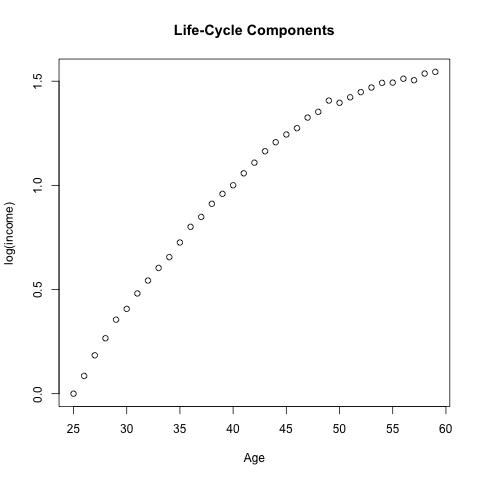
\includegraphics[scale=.5]{age}

\pagebreak

 The estimated cohort components are plotted below:

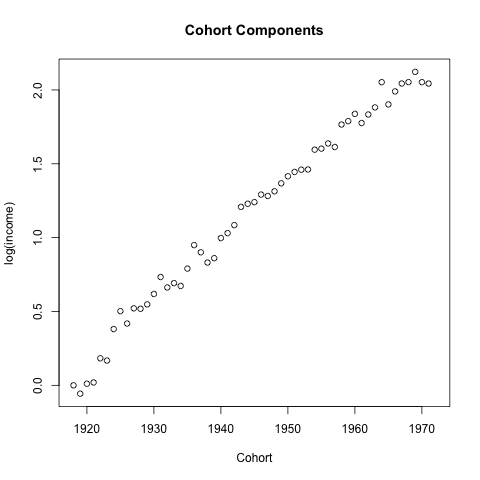
\includegraphics[scale=.5]{cohort}


\item Taking $\varepsilon_{i,t}$, I compute pseudo differences using $\rho = 0.97$:

$$
\tilde{\Delta} y_{i,t} = \varepsilon_{i,t} - \rho \varepsilon_{i,t-1}
$$

\item Then estimate $\sigma_\varepsilon^2$ and $\sigma_\zeta^2$ using the following formulas:


\begin{align*}
\hat{\sigma}_\varepsilon^2 &= \frac{-1}{\rho} Cov(\tilde{\Delta} y_{i,t}, \tilde{\Delta} y_{i,t+1})\\
\hat{\sigma}_\zeta^2 &= \frac{1}{\rho} Cov(\tilde{\Delta} y_{i,t}, \rho^2 \tilde{\Delta} y_{i,t-1} + \rho \tilde{\Delta} y_{i,t} + \tilde{\Delta} y_{i,t-1})
\end{align*}

\item The resulting point estimates are 

\begin{center}
\begin{tabular}{ l | r}
& Data Moment\\
\hline
$\hat{\sigma}_\varepsilon^2$  & 0.0563 \\  
$\hat{\sigma}_\zeta^2$ & 0.0673
\end{tabular}
\end{center}

\item See \texttt{part\_1.R} for the implementation.

\pagebreak

\section{Part 2: Model}

\item Some details about I implemented the model:

\begin{itemize}

\item The life-cycle component is estimate in the part 1.  I use the age fixed effects (see Life-Cycle Components figure) plus the intercept of 8.14951

\item There's a zero borrowing limit.

\item The asset grid goes from \$0 to \$2,000,000 with 500 grid points.

\item Tauchen is used to discretize the persistent income shock with 5 states (using \texttt{tauchen} function from QuantEcon).

\item The transitory income shock has 5 states.

\item The model is simulated for 5000 individuals.

\end{itemize}

\item The graph of average wealth by age is below:

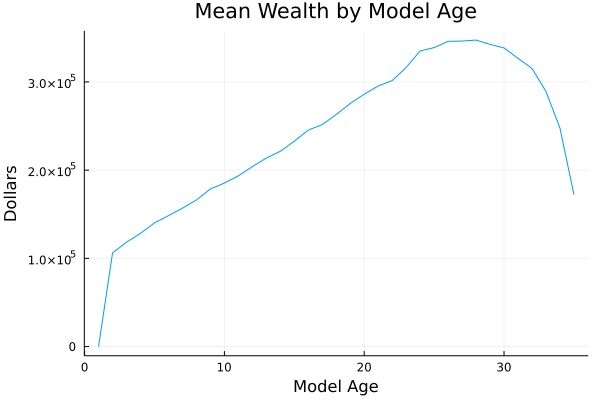
\includegraphics[scale=.5]{mean_wealth}

\pagebreak

\item The graph of consumption variance by age is below:

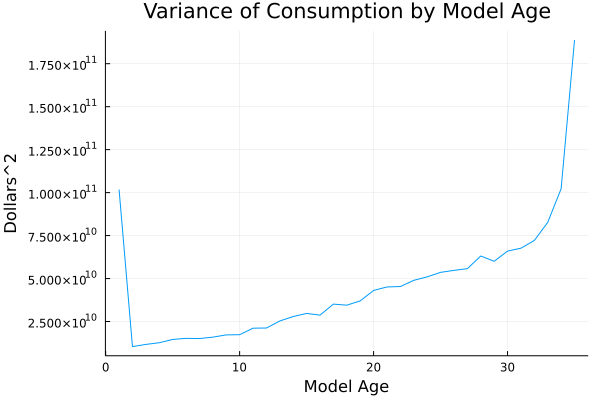
\includegraphics[scale=.5]{var_consumption}

\item My results for the passthrough of the shocks are off, so I'm not reporting them here. I think there's a bug somewhere, but my time constraint is binding.

\item A comparison of the variance of the shocks from the data and then recovered from the model simulation (calibrated to the data moment).  Consistent with Kaplan and Violante, the implied $\hat{\sigma}_\varepsilon^2$ is pretty close, but the implied $\hat{\sigma}_\zeta^2$ is relatively small.

\begin{center}
\begin{tabular}{ l | r | r}
                              & Data Moment   & Simulation Moment \\  
\hline
$\hat{\sigma}_\varepsilon^2$  & 0.0563 & 0.0625 \\  
$\hat{\sigma}_\zeta^2$        & 0.0673 & 0.0196
\end{tabular}
\end{center}

\item See the Julia scripts for the implementation:

\begin{itemize}
\item \texttt{part\_2\_model.jl} contains code for solving the model.
\item \texttt{part\_2\_simulation.jl} contains code for simulating the model and manipulating the simulation results.
\item \texttt{part\_2\_run.jl} runs the analysis and creates figures.
\end{itemize}

\end{itemize}

\end{document}

